%Every piece of package I've acumulated over the last years
%
%
\documentclass[a4paper,12pt]{article}
\usepackage[spanish]{babel}
\usepackage[utf8]{inputenc}
\usepackage{imakeidx}
\usepackage{graphicx}
\usepackage{float}
\usepackage{amsmath}
\usepackage[backend=bibtex,style=verbose]{biblatex}
\bibliography{bibliography}
\usepackage{csquotes}
\usepackage{tcolorbox}
\usepackage{multirow}
\usepackage{caption}
\usepackage{subcaption}
\usepackage{afterpage}
\usepackage{blindtext}

\usepackage[margin=0.5in]{geometry}
%End of packages
%
%
%
\begin{document}

\title{Análisis de Diodos}
\author{Gabriel D'Andrade Furlanetto}
\maketitle

\abstract{En este artigo, vamos analizar la tensión umbral de diferentes diodos utilizando datos coletados con la herramienta de instrumentación virtual LabView. Analizaremos también un Diodo Zener y su tensión Zener con la misma metodología.}

\section{Introducción}

\subsection{Objetivos}
Queremos aqui, principalmente, caracterizar diferentes diodos por sus tensiones umbrales. Especificamente, vamos a analizar 8 diodos diferentes:LED Amarillo,LED Azul, LED Blanco, LED Verde, LED Rojo, LED Infrarojo, Diodo PV, Diodo Zener. Para este último, también queremos caracterizar su tensión Zener

\subsection{Conceptos básicos del montaje experimental}
Para lo que queremos hacer y caracterizar, necesitamos producir curvas $I-V$ para los diferentes diodos. La forma más sencilla de hacer eso sería variando la corriente y midiendo la diferencia de potencial entre los terminales del diodo. No obstante, no podemos directamente variar la intensidad directamente con nuestros aparatos.

De esa manera, controlaremos la tensión de entrada, $V_0$, utilizando la resistencia que tenemos para calcular la corriente, y mediremos la diferencia de potencial entre los terminales del diodo. El circuito está representado en la Figura \ref{diagrama}

\begin{figure}[H]
	\centering
	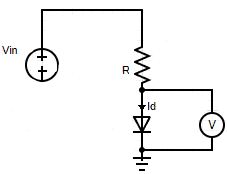
\includegraphics[width=0.2\textwidth]{diagram.jpg}
	\caption{Diagrama del circuito del montaje experimental.}
	\label{diagrama}
\end{figure}


\section{Procedimiento Experimental}



\subsection{Programa de Labview}
El programa, formalmente el VI, utilizado para las mediciones consiste en un panel frontal, que existe principalmente para indicar si la medición va bien y controlar el número de muestras, la resistencia y los valores finales y iniciales de la tensión, y un panel trasero que, funcionalmente, es donde las mediciones y transformaciones relevantes ocurren. El programa está diseñado para hacer el output a un archivo para que un análisis completo pueda ser hecho en otros medios, y está integralmente representado en la Figura \ref{fig:combined}.

El código del panel trasero basicamente hace un gradiente con el número de muestras que va de la voltaje inicial a la final. El bucle $for$ pasa por cada uno de esos valores (uno a cada 20 ms) y para cada uno de eses, hace pasar esa tensión como $V_{0}$ al circuito. Despúes, se mide el voltaje de salida, $V_{Out}$ y, con la resistencia y matemáticas básica, calcula el valor de la intensidad. Finalmente, hace el display del gráfico en el panel frontal y el output de los valores a un archivo de texto para que se puedan analizar en programas diseñados para este fin. Tambien reseteamos el valor de la tensión inicial a 0 después de la ejecución del bucle para no dejarlo encencidido.

\begin{figure}
	\begin{subfigure}{\textwidth}
		\centering
		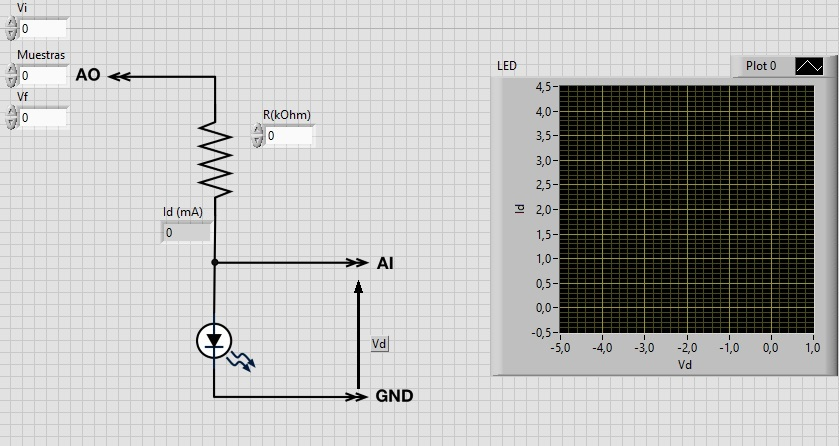
\includegraphics[width = 0.6\textwidth]{front.jpg}
		\caption{Panel frontal del VI.}
		\centering
	\end{subfigure}


	\begin{subfigure}{\textwidth}
		\centering
		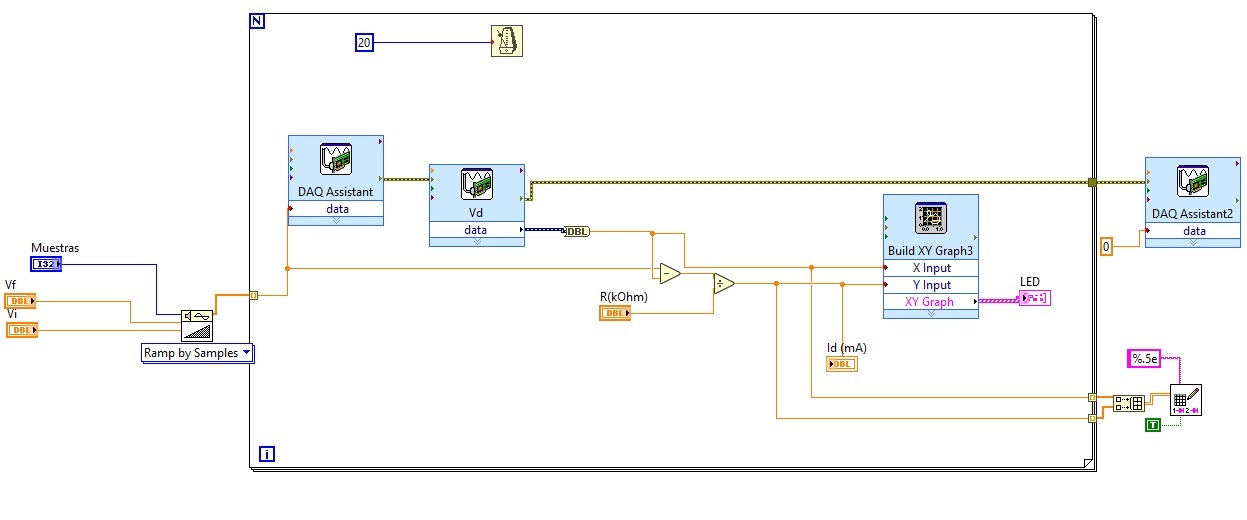
\includegraphics[width = \textwidth]{back.jpg}
		\caption{Panel trasero del VI.}
		\label{fig:right}
	\end{subfigure}

	\caption{El VI utilizado para las mediciones.}
	\label{fig:combined}
\end{figure}
\subsection{Medidas}
Despúes de hacer las medidas y procesarlas en un software estándar, tenemos los resultados representados en la Figura \ref{3}
\begin{figure}[H]
	\begin{subfigure}{0.49\textwidth}
		\label{Diodos}
		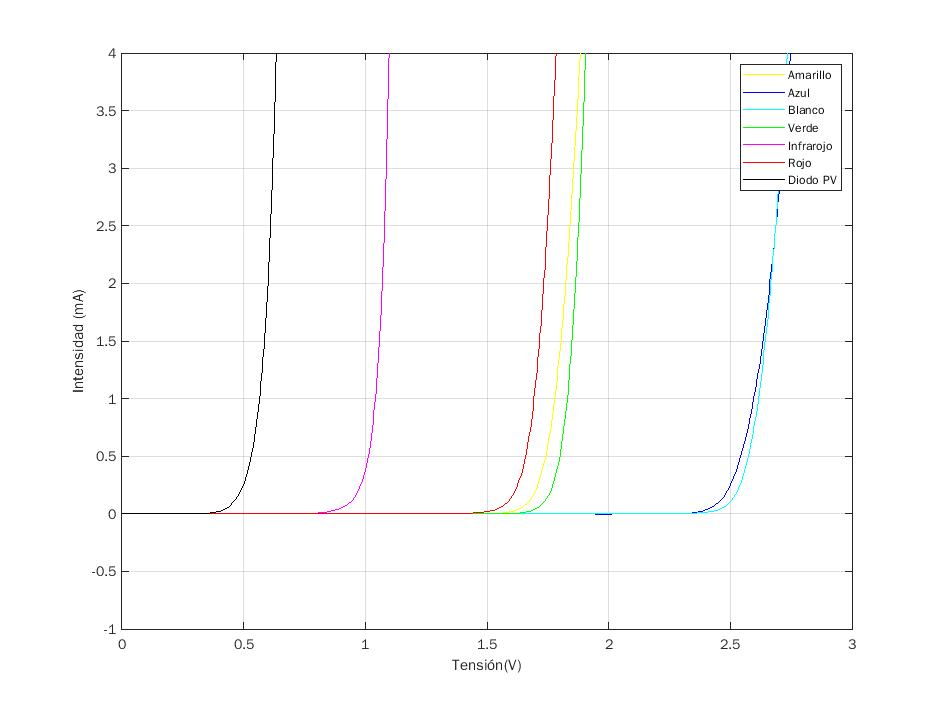
\includegraphics[width=.9\textwidth]{diodos.jpg}
		\centering
		\caption{Intensidad como función de la diferencia de potencial entre extremos de diferentes diodos.}	
	\end{subfigure}
\begin{subfigure}{0.49\textwidth}
	\centering
	\label{zener}
	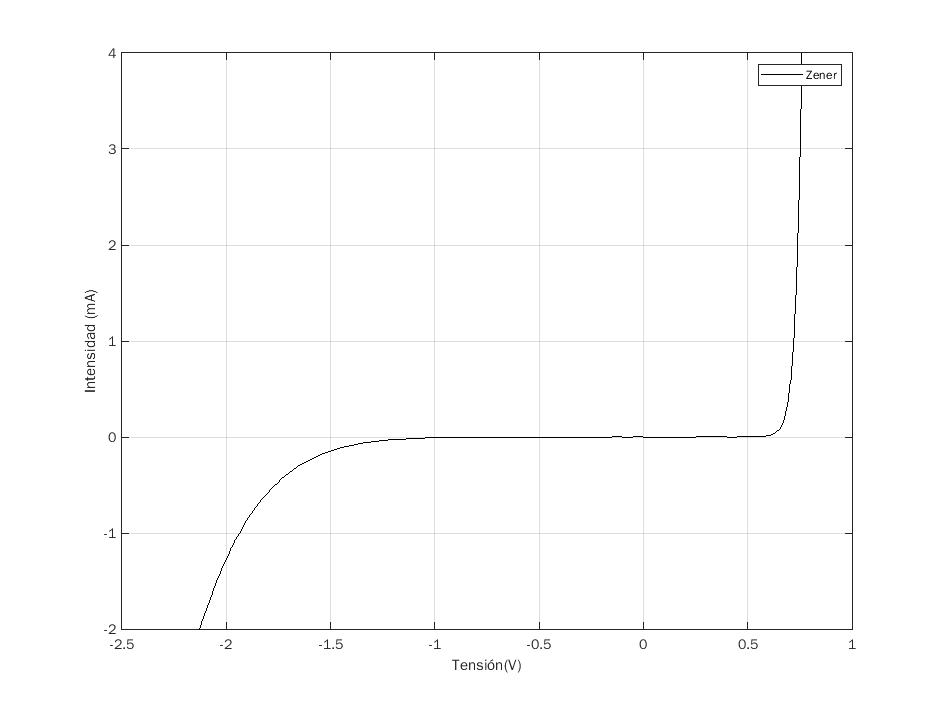
\includegraphics[width=.9\textwidth]{zener.jpg}
	\caption{Intensidad como función de la diferencia de potencial entre extremos del diodo zener.}
\end{subfigure}
\caption{Mediciones hechas durante el experimento.}\label{3}
\end{figure}


\section{Resultados}
Utilizando los datos que usamos para hacer la Figura 3, podemos trivialmente calcular la tension umbral para los differentes diodos y la tensión de Zener del diodo Zener:
\begin{gather*}
	V_{PV} = 0.63 \text{V}\\
	V_{Infrarojo} = 1.10 \text{V} \\
	V_{Rojo} = 1.78 \text{V} \\
	V_{Amarillo} = 1.90 \text{V} \\
	V_{Verde} = 1.92 \text{V}\\
	V_{Blanco} = 2.73 \text{V} \\
	V_{Azul} = 2.75 \text{V}\\ 
	V_{UmbZen} = 0.75 \text{V}\\
	V_{ZenZen} = -2.21\text{V}
\end{gather*}

Los LEDs aqui presentan el comportamiento esperado: Su tensión umbral es proporcional a la frecuencia de la luz emitida.

\section{Discusión Final}
Hemos podido cumplir todos los objetivos propuestos y medir las tensiones deseadas para cada uno de los diodos. Más allá, hemos verificado que la relación teórica de proporcionalidad de los LEDs y sus tensiones umbrales se verifica, ilustrando la validad de nuestro experimento.
\end{document}